\documentclass[
	draftmark = false,
%	traditional = true,
%	colors = false,
%	coverpage = coverpage.tex,
%	coverpage = coverpage.pdf,
%   geometry = b5,
	fontsetup = font-setup-open.tex,
	titlesetup = titles-setup.tex
]{AJbook}

\usepackage[xindy, splitindex]{imakeidx}
\makeindex[
	columns=2,
	program=truexindy,
	intoc=true,
	options=-M texindy -I xelatex -C utf8,
	title={名词索引}]	% 名词索引

\usepackage[unicode, bookmarksnumbered]{hyperref}
\hypersetup{
	pdfauthor = {Lyscoria},
	pdftitle = {信数笔记},
	CJKbookmarks = true}

% 增加表格高度
\renewcommand*\arraystretch{1.5}

% 图片相关的宏包
\usepackage{graphicx} %插入图片的宏包
\usepackage{float} %设置图片浮动位置的宏包
\usepackage{subfigure} %插入多图时用子图显示的宏包

\numberwithin{equation}{section}
\renewcommand{\theequation}{\thesection--\arabic{equation}}

\numberwithin{figure}{section}
\renewcommand{\thefigure}{\thechapter--\arabic{figure}}

\numberwithin{table}{section}
\renewcommand{\thetable}{\thechapter--\arabic{table}}

% 算法相关宏包
\usepackage{algorithm}      % 提供浮动体环境（外面的框和标题）
\usepackage{algpseudocode}  % 提供伪代码命令（里面的 \State, \If 等）

% 绘图
\usepackage{tikz}
\usepackage{pgfplots}
\pgfplotsset{compat=1.18}

\usepackage{enumitem}

\renewcommand{\d}{\mathrm{d}}   % 微分符号
\newcommand{\e}{\mathrm{e}}     % e
\newcommand{\E}{\mathbb{E}}     % 期望
\newcommand{\Var}{\text{Var}}   % 方差
\newcommand{\Cor}{\text{Cor}}   % 协方差
\newcommand{\sign}{\text{sign}} % 符号函数
\newcommand{\Err}{\text{Err}}   % 误差

\allowdisplaybreaks[4]

\begin{document}

    \frontmatter

    \mainmatter

    \chapter{高维几何}

\section{在高维单位球中采样}

我们用 $V(d,r)$ 表示 $\mathbb{R}^{d}$ 中的半径为 $r$ 的球的体积，单位球的体积则简记作 $V(d)$。易见：
\[
	V(d,r) = r^{d} \cdot V(d)
\]
在接下来的部分中，我们会多次遇到“从单位球中随机取一个点”的说法，所以我们需要弄清怎样在 $d$ 维单位球中均匀地采样。先考虑如何在球的表面均匀采样：

\begin{algorithm}[h]
    \caption{单位球表面的采样}
    \begin{algorithmic}[1]
        \For{$i = 1$ to $d$}
            \State 独立地从标准高斯分布中采样 $x_i \sim N(0, 1)$
        \EndFor
        \State $x = (x_1, \dots, x_d)$
        \State $x \leftarrow \dfrac{x}{\|x\|}$
        \State \Return $x$
    \end{algorithmic}
\end{algorithm}

为什么这个算法是 work 的？回忆高斯分布的概率密度函数，有
\[
	p(x_{i}) \propto \exp\left(-\frac{1}{2}x_{i}^{2}\right)
\]
\[
	p(x_{1}, \dots, x_{d}) \propto \prod_{i=1}^{d} \exp\left(-\frac{1}{2}x_{i}^{2}\right) = \exp\left(-\frac{1}{2}\sum x_{i}^{2}\right) = \exp\left(-\frac{1}{2}\|x\|^{2}\right)
\]

概率仅与 $\|x\|$ 有关，所以得到的点在球面上是均匀分布的。接下来，为了在整个球上采样，只需要把表面上的点“缩放”到整个球中即可。易知球表面积正比于 $r^{d-1}$，令 $p(r) = c \cdot r^{d-1}$，积分 $\int c r^{d-1} = 1 \Rightarrow c=d$，由此得到：

\begin{algorithm}[h]
    \caption{单位球中的采样}
    \begin{algorithmic}[1]
        \For{$i = 1$ to $d$}
            \State 从标准高斯分布中采样 $x_i \sim N(0, 1)$
        \EndFor
        \State $x = (x_1, \dots, x_d) / \|x\|$
        \State 从 $p(r) = d r^{d-1}$ 中采样 $r$
        \State \Return $rx$
    \end{algorithmic}
\end{algorithm}

\section{高维单位球的体积}

本节来推导 $V(d)$ 的具体表达式。引入 $A(d,r)$ 和 $A(d)$ 来表示表面积。

\begin{lemma}
    单位球体积和表面积有如下关系：
    \[
        V(d) = \frac{A(d)}{d}
    \]
\end{lemma}

\begin{proof}
    \[
        V(d)=\int_{0}^{1}A(d,r)\d r=A(d)\int_{0}^{1}r^{d-1}\d r = \frac{A(d)}{d}
    \]
\end{proof}

\begin{lemma}
    \[
        \int_{-\infty}^{+\infty}{\e}^{-x^{2}}dx=\sqrt{\pi}
    \]
\end{lemma}

\begin{proof}
    首先有
    \begin{align*}
        \left(\int_{-\infty}^{+\infty}{\e}^{-x^{2}}\d x\right)^{2} &= \left(\int_{-\infty}^{+\infty}{\e}^{-x^{2}}\d x\right)\left(\int_{-\infty}^{+\infty}{\e}^{-y^{2}}\d y\right) \\
        &= \int_{-\infty}^{+\infty}\int_{-\infty}^{+\infty}{\e}^{-(x^{2}+y^{2})}\d x\d y
    \end{align*}
    从几何上看，整个体积可以当作对底面半径为 $r$，高为 $\e^{-r^2}$ 的圆柱面的累加：

    \begin{figure}[htbp]
        \centering
        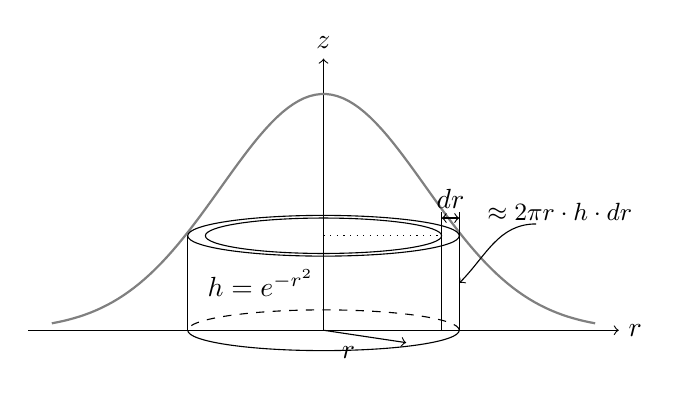
\begin{tikzpicture}[scale=1.5]
           
            \def\H{2.0}        
            \def\R{1.0}        
            \def\dR{0.15}      
            \def\ShellH{0.8}   
            \def\Y{0.15}      
    
            \draw[->] (-2.5, 0) -- (2.5, 0) node[right] {$r$};
            \draw[->] (0, 0) -- (0, \H+0.3) node[above] {$z$};
    
            \draw[gray, thick] plot[domain=-2.3:2.3, samples=100] (\x, {\H*exp(-\x*\x/1.5)});
            
            \draw[black, dashed] (\R+\dR, 0) arc (0:180:{\R+\dR} and {(\R+\dR)*\Y});

            \draw[black] (\R+\dR, 0) arc (0:-180:{\R+\dR} and {(\R+\dR)*\Y});
    
            \draw[black] (0, \ShellH) ellipse ({\R} and {\R*\Y});
            \draw[black] (0, \ShellH) ellipse ({\R+\dR} and {(\R+\dR)*\Y});
    
            \draw[black] (-\R-\dR, 0) -- (-\R-\dR, \ShellH);
            \draw[black] (\R, 0) -- (\R, \ShellH);
            \draw[black] (\R+\dR, 0) -- (\R+\dR, \ShellH);
    
            \draw[black, ->] (0, 0) -- (0.7*\R, -0.7*\R*\Y) node[midway, below left] {$r$};
            
            \draw[black] (\R, \ShellH) -- (\R, \ShellH+0.2);
            \draw[black] (\R+\dR, \ShellH) -- (\R+\dR, \ShellH+0.2);
            \draw[black, <->] (\R, \ShellH+0.15) -- (\R+\dR, \ShellH+0.15) node[midway, above] {$dr$};
            
            \draw[black, dashed] (0, 0) -- (0, \ShellH);
            \draw[black, dotted] (0, \ShellH) -- (\R, \ShellH);
            \node at (0, \ShellH/2) [left] {$h = e^{-r^2}$};
    
            \node at (2.0, 1.0) [align=left] {\small  $\approx 2\pi r \cdot h \cdot dr$};
            \draw[->, thin] (1.8, 0.9) to[out=180, in=45] (\R+\dR, \ShellH/2);
    
        \end{tikzpicture}
        \caption{高斯积分}
    \end{figure}

    于是
    \begin{align*}
        \int_{-\infty}^{+\infty}\int_{-\infty}^{+\infty}{\e}^{-(x^{2}+y^{2})}\d x\d y &= \int_{0}^{+\infty}{\e}^{-r^{2}} \cdot 2\pi r \d r \\
        &= \pi\int_{0}^{+\infty}{\e}^{-r^{2}}\d r^{2} \\
        &= \pi(-{\e}^{-r^{2}})\Big|_{0}^{+\infty} \\
        &= \pi
    \end{align*}
    从而原积分等于 $\sqrt{\pi}$。
\end{proof}

下面我们来计算 $V(d)$。方法是通过两种方式来计算积分：
\[
    \int_{-\infty}^{+\infty}\int_{-\infty}^{+\infty}\dots\int_{-\infty}^{+\infty}\e^{-(x_{1}^{2}+\dots+x_{d}^{2})}\d x_{1}\dots \d x_{d}
\]

一方面，利用之前的结果，上面的积分正是
\[
	\left(\int_{-\infty}^{+\infty}\e^{-x^{2}}\d x\right)^{d}=\pi^{\frac{d}{2}}
\]

另一方面，仍从几何上来看。令 $r^{2}=x_{1}^{2}+\dots+x_{d}^{2}$，整个体积依然是底面半径为 $r$ 的圆柱面的累加，只不过这里圆柱面的底面圆从 $2$ 维变成了 $d$ 维的。
\begin{align*}
	&\int_{-\infty}^{+\infty}\dots\int_{-\infty}^{+\infty}\e^{-(x_{1}^{2}+\dots+x_{d}^{2})}\d x_{1}\dots \d x_{d} \\
	= &\int_{0}^{+\infty}\e^{-r^{2}}\cdot A(d,r) \d r \\
    = &A(d) \int_{0}^{+\infty}\e^{-r^{2}}r^{d-1}\d r
\end{align*}

形如 $\displaystyle \int_0^{+\infty} x^n \e^{-x} \d x$ 的积分比较特别：
\begin{align*}
	\int_0^{+\infty} x^n \e^{-x} \d x &= \int_0^{+\infty} x^n \d(-\e^{-x}) \\
	&= -x^n \e^{-x} \bigg|_0^{+\infty} + \int_0^{+\infty} \e^{-x} \d x^n \\
	&= n \int_0^{+\infty} x^{n-1} \e^{-x} \d x
\end{align*}

令 $\Gamma(t+1) = \displaystyle \int_0^{+\infty} x^t \e^{-x} \d x$，则 $\Gamma(t+1) = t\Gamma(t)$，因而它是阶乘的推广。回到上面，由于
\begin{align*}
    \int_{0}^{+\infty}\e^{-r^{2}}r^{d-1}\d r &= \int_{0}^{+\infty}\e^{-r^{2}}(r^{2})^{\frac{d-1}{2}}\d r \\
    &= \int_{0}^{+\infty}\e^{-t} t^{\frac{d-1}{2}} \frac{1}{2} t^{-\frac{1}{2}} \d t \\
    &= \frac{1}{2}\int_{0}^{+\infty}\e^{-t}t^{\frac{d}{2}-1}\d t \\
	&= \frac{1}{2}\Gamma\left(\frac{d}{2}\right)
\end{align*}

所以
\[
    \pi^{\frac{d}{2}}=A(d)\cdot\frac{1}{2}\Gamma\left(\frac{d}{2}\right)
\]

由此得到结论：

\begin{theorem}
$d$ 维单位球的表面积和体积公式：
\[
	A(d)=\frac{2\pi^{\frac{d}{2}}}{\Gamma(\frac{d}{2})}
\]
\[
	V(d)=\frac{\pi^{\frac{d}{2}}}{\frac{d}{2}\Gamma(\frac{d}{2})}
\]
\end{theorem}

\section{高维单位球的更多性质}

\subsection{体积趋于0}

\begin{theorem}
    $d$ 维单位球的体积最终趋于 $0$，
    \[\lim_{d \to \infty} V(d) = 0\]
\end{theorem}

\begin{proof}
    使用 Stirling 公式，略。
\end{proof}

\subsection{体积集中在表面}

\begin{theorem}
    设 $S$ 为单位球，$(1-\epsilon)S=\{(1-\epsilon)x|x\in S\}$。
则至少有 $1-\e^{-\epsilon d}$ 比例的体积分布在 $S \setminus (1-\epsilon)S$ （“球壳”）中。
\end{theorem}

\begin{proof}
    \[
	   \frac{V((1-\epsilon)S)}{V(S)}=(1-\epsilon)^{d}\le \e^{-\epsilon d}
    \]
\end{proof}

\subsection{体积集中在“赤道”}

\begin{theorem}
    对 $c\ge1, d\ge3$，至少有 $1-\frac{2}{c}\e^{-\frac{c^{2}}{2}}$ 比例的体积满足 $|x^{(1)}|\le\frac{c}{\sqrt{d-1}}$。
\end{theorem}

\begin{proof}
    记 $S$ 为单位球。待定 $h \in (0, 1)$，令
    \[
	   H=\{x\in S \mid x^{(1)}\ge 0\}
    \]
    \[
	   A=\{x\in S \mid x^{(1)}\ge h\}
    \]

    \begin{figure}[htbp]
        \centering
        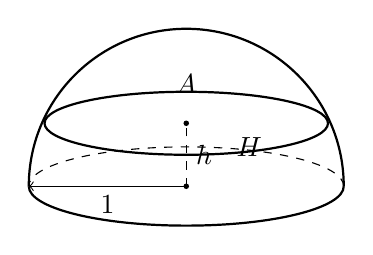
\begin{tikzpicture}[scale=1]
            \def\R{2} 
            \def\H{0.8}
            \def\r{1.8} 
            
            \draw[dashed] (\R,0) arc (0:180:{\R} and {0.5});
            \draw[thick] (\R,0) arc (0:-180:{\R} and {0.5});
            \draw[thick] (\R,0) arc (0:180:\R);
            \draw[thick] (0,\H) ellipse ({\r} and {0.4});
            
            \draw[dashed] (0,0) -- (0,\H) node[midway, right] {$h$};
            \fill (0,0) circle (1pt);
            \fill (0,\H) circle (1pt);

            \draw[->] (0,0) -- (-\R, 0) node[midway, below] {$1$};
            \node at (0, \H+0.5) {$A$};
            \node at (0.8, 0.5) {$H$};
        \end{tikzpicture}
        \caption{$H$ 与 $A$}
    \end{figure}
    
    先来放缩 $A$ 的体积：
    \begin{align*}
    	V(A) &= \int_{h}^{1}V(d-1,\sqrt{1-x^{2}})\d x \\
    	&= V(d-1)\int_{h}^{1}(1-x^{2})^{\frac{d-1}{2}}\d x \\
        &\le V(d-1)\int_{h}^{1}\e^{-\frac{d-1}{2}x^{2}}\d x \\
    	&\le V(d-1)\int_{h}^{+\infty}\frac{x}{h}\e^{-\frac{d-1}{2}x^{2}}\d x \\
    	&= \frac{V(d-1)}{h}\int_{h}^{+\infty}\e^{-\frac{d-1}{2}x^{2}}\d\left(\frac{x^{2}}{2}\right) \\
        &= \frac{V(d-1)}{h(d-1)}\e^{-\frac{d-1}{2}h^{2}}
    \end{align*}
    
    下面考虑 $H$ 的体积（$H$ 已经有了明确表达式为什么还要放缩？我们希望有一个包含 $V(d-1)$ 的界来和上面的消掉）。

    \begin{figure}[htbp]
        \centering
        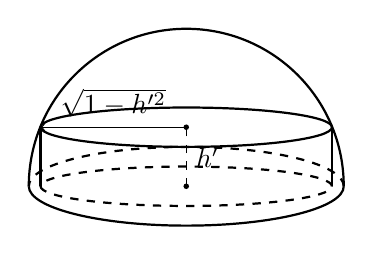
\begin{tikzpicture}[scale=1]
            \def\R{2}
            \def\H{0.75}
            \def\r{1.85}
            
            \draw[black, dashed, thick] (\R,0) arc (0:180:{\R} and {0.5});
            \draw[black, thick] (\R,0) arc (0:-180:{\R} and {0.5});
            \draw[black, thick] (\R,0) arc (0:180:\R);
            
            \draw[black, thick] (0,\H) ellipse ({\r} and {0.25});
            \draw[black, dashed, thick] (0,0) ellipse ({\r} and {0.25});
            \draw[black, thick] (-\r, 0) -- (-\r, \H);
            \draw[black, thick] (\r, 0) -- (\r, \H);
            
            \draw[black, dashed] (0,0) -- (0,\H) node[midway, right] {$h'$};
            \fill[black] (0,0) circle (1pt);
            \fill[black] (0,\H) circle (1pt);
            \draw[black, ->] (0,\H) -- (-\r, \H) node[midway, above] {$\sqrt{1-h'^2}$};
            
        \end{tikzpicture}
        \caption{$H$}
    \end{figure}
    
    如图所示， $V(H)$ 一定大于等于高为 $h'$ 的圆柱的体积（$h'$ 也待定），这样就有
    \begin{align*}
    	V(H) &\ge V(d-1,\sqrt{1-h'^{2}})\cdot h' = V(d-1)(1-h'^{2})^{\frac{d-1}{2}}h' \\
    	&\ge V(d-1)\left(1-\frac{d-1}{2}h'^{2}\right)h'
    \end{align*}
    令 $h=\frac{c}{\sqrt{d-1}}$, $h'=\frac{1}{\sqrt{d-1}}$，则有：
    \begin{align*}
    	V(A) &\le\frac{V(d-1)}{c\sqrt{d-1}}\e^{-\frac{c^{2}}{2}} \\
    	V(H) &\ge V(d-1)\cdot\left(1-\frac{1}{d-1}\cdot\frac{d-1}{2}\right)\cdot\frac{1}{\sqrt{d-1}}=\frac{V(d-1)}{2\sqrt{d-1}}
    \end{align*}
    综上可得：
    \[
    	\frac{V(A)}{V(H)}\le\frac{2}{c}\e^{-\frac{c^{2}}{2}}
    \]
\end{proof}

\subsection{球上的点几乎两两正交}

\begin{theorem}
    在单位球中随机取 $n$ 个点 $x_1, \dots, x_n$, 有 $1 - O(\frac{1}{n})$ 的概率使得
    \begin{enumerate}
    	\item $\|x_i\| \ge 1 - \frac{2 \ln n}{d} \quad \forall i$.
    	\item $|\langle x_i, x_j \rangle| \le \frac{\sqrt{6 \ln n}}{\sqrt{d-1}} \quad \forall i \neq j$.
    \end{enumerate}
\end{theorem}

\begin{proof}
    利用 Union Bound.
    \begin{align*}
    	\Pr\left[\exists i, \|x_i\| < 1-c\right] &\le n \Pr\left[\|x_1\| < 1-c\right] \\
    	&= n \cdot (1-c)^d < n \e^{-cd}
    \end{align*}
    只要使 $n \e^{-cd} \le \frac{1}{n}$ 即可, 取 $c = \frac{2 \ln n}{d}$.
    
    对于第二个不等式, 将 $x_1$ 旋转到 $(1, 0, \dots, 0)$ 所在的方向, 则 $|\langle x_1, x_j \rangle| \le |x_j^{(1)}|$. 利用刚刚的结果，
    \begin{align*}
    	\therefore \Pr\left[\exists i \neq j, |\langle x_i, x_j \rangle| > \frac{c}{\sqrt{d-1}}\right] 
    	&\le n^2 \Pr\left[|\langle x_1, x_2 \rangle| > \frac{c}{\sqrt{d-1}}\right] \\
    	&\le n^2 \Pr\left[|x_1^{(1)}| > \frac{c}{\sqrt{d-1}}\right] \\
    	&\le n^2 \cdot \frac{2}{c} \e^{-\frac{c^2}{2}} \\
    	&\le n^2 \e^{-\frac{c^2}{2}}
    \end{align*}
    只要让 $n^2 \e^{-\frac{c^2}{2}} \le \frac{1}{n}$, 即 $\e^{-\frac{c^2}{2}} \le \frac{1}{n^3}$.
    取 $c = \sqrt{6 \ln n}$ 即可.
\end{proof}

\subsection{体积集中在中心的立方体内}

\begin{theorem}
    单位球至少一半的体积集中在中心在原点的边长 $\frac{4\sqrt{\ln d}}{\sqrt{d-1}}$ 的正方体内部。
\end{theorem}

\begin{proof}
    \[
    	\Pr\left[\exists i, |x^{(i)}| > \frac{c}{\sqrt{d-1}}\right] \le d\cdot\frac{2}{c}\e^{-\frac{c^{2}}{2}}
    \]
    取 $c=2\sqrt{\ln d}$，则上界为 $d \cdot \frac{1}{\sqrt{\ln d}}\cdot\frac{1}{d^{2}} < \frac{1}{d} < \frac{1}{2}$。
\end{proof}

这也为 $V(d)\rightarrow 0$ 提供了另一种证明。

注：看上去与球的体积集中在表面矛盾？实际上这个立方体在 $d$ 较大的时候并不是完全位于球的内部的，会伸出来很多“刺”，类似于一个“海胆”，参见书上的这幅图：

\begin{figure}
    \centering
    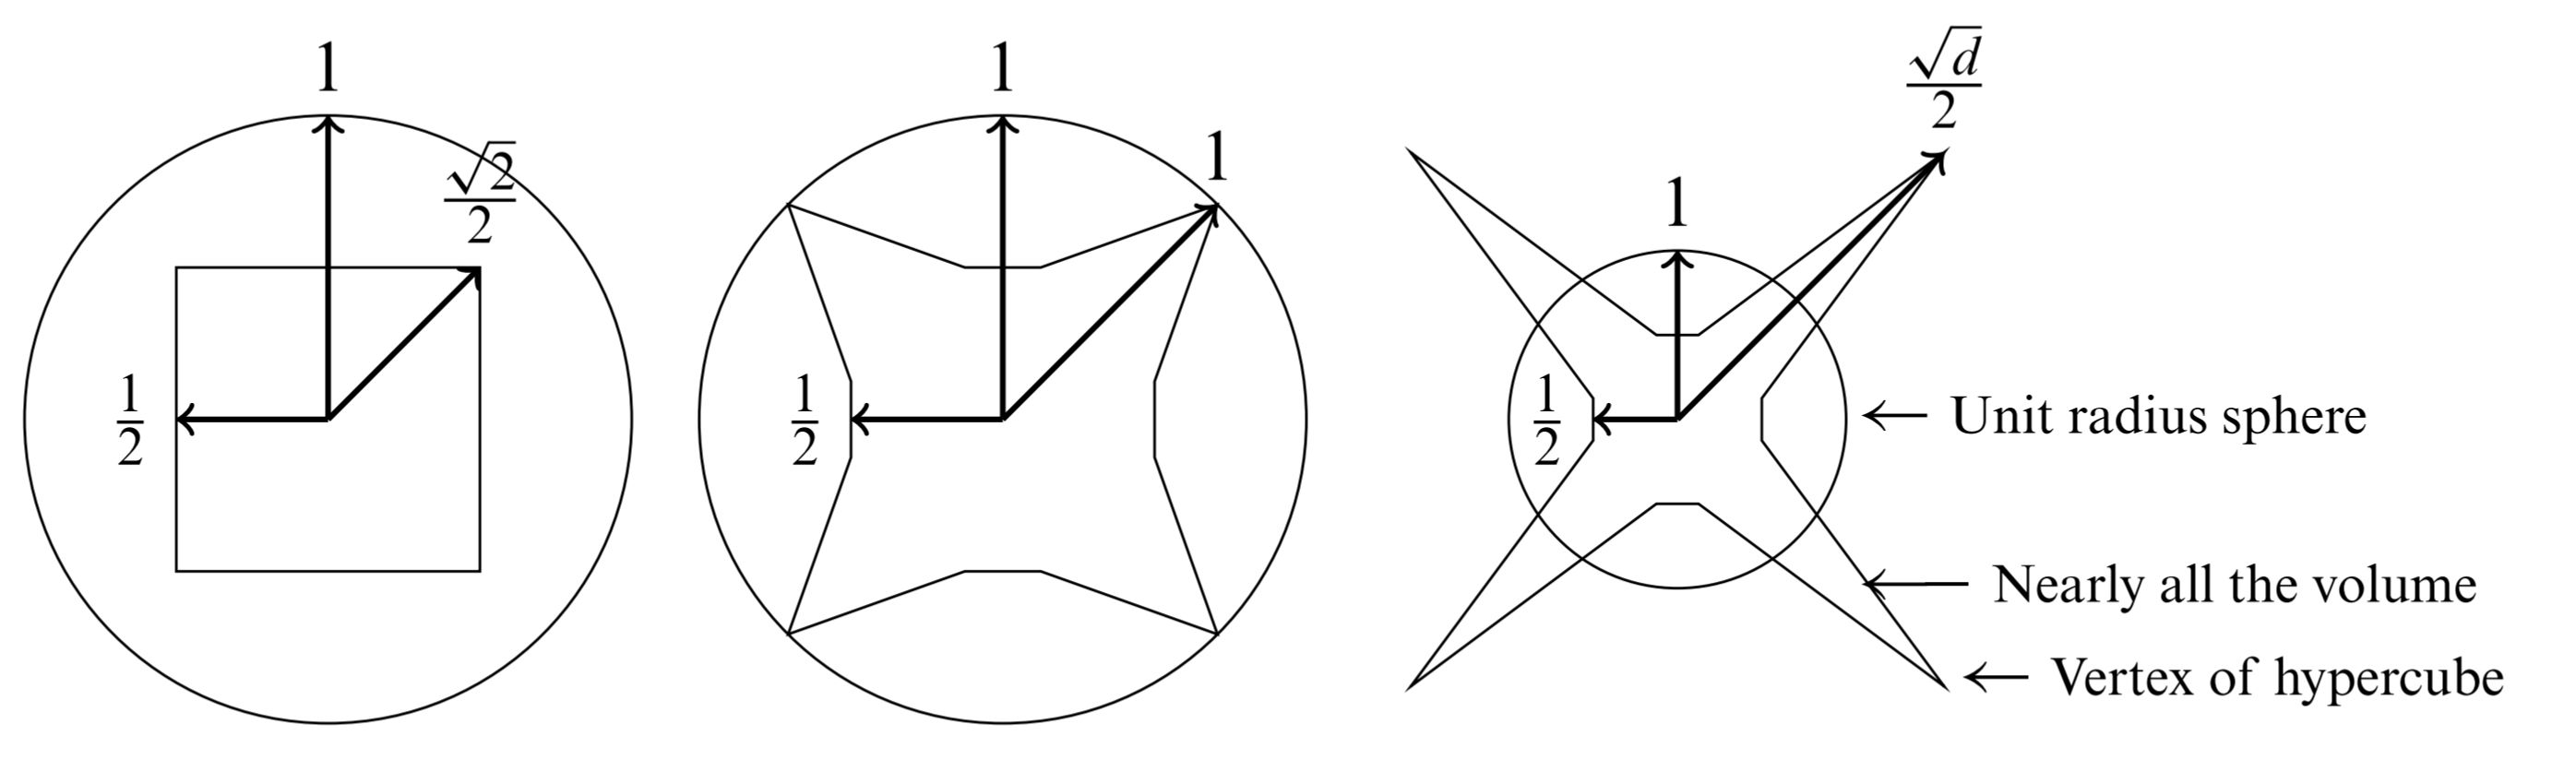
\includegraphics[width=1.0\linewidth]{imgs/sphere_and_cube.jpg}
    \caption{$2$, $4$, $d$ 维的球面与立方体的示意图}
\end{figure}

\section{随机投影，Johnson-Lindenstrauss 引理}

先简单引入一个工具：

\begin{theorem}
    对任意正整数 $d$，独立地从标准高斯中采样 $x=(x_{1},\dots,x_{d})$，则存在正常数 $c$，使得对 $\beta\le\sqrt{d}$，至少有 $1-3\e^{-c\beta^{2}}$ 的概率使
    \[
    	\|x\| \in [\sqrt{d}-\beta, \sqrt{d}+\beta].
    \]
\end{theorem}

这个定理称为“高斯圆环定理”，此处不证。其实很符合直觉：$\E[\|x\|^{2}]=\E[x_{1}^{2}+\dots+x_{d}^{2}]=d\E[x_{1}^{2}]=d$，故 $x$ 大概率分布在半径 $\sqrt{d}$ 附近的“圆环”中。

接下来我们关心这样一件事情，对于 $k \ll d$，给定 $\mathbb{R}^{d}$ 中的 $n$ 个点 $v_{1}, \dots, v_{n}$，能否找到一个投影 $f: \mathbb{R}^{d}\longrightarrow \mathbb{R}^{k}$ 使得在降维的同时尽量保持这 $n$ 个点间的距离？
也即对 $\epsilon\in(0,1)$，$\forall i,j$：
\[
	(1-\epsilon)\|v_{i}-v_{j}\| \le \|f(v_{i})-f(v_{j})\| \le (1+\epsilon)\|v_{i}-v_{j}\| ?
\]

为了解决这件事，我们需要使用所谓的\textbf{概率方法}：要证明存在满足性质 $P(x)$ 的对象 $x$，只要证明以某种方式随机取 $x$，$\Pr[P(x)]>0$ 即可。

如何来构造这种随机？我们利用标准高斯分布，随机选取 $u_{1},\dots,u_{k} \in \mathbb{R}^{d}$ i.i.d $\sim N(0,1)$。定义 $f: \mathbb{R}^{d}\longrightarrow\mathbb{R}^{k}$，
\[
	v \mapsto (\langle v,u_{1}\rangle, \dots, \langle v,u_{k}\rangle)
\]
我们可以证明，这样的 $f$ 大概率能把距离保持地很好：

\begin{theorem}
    对于 $0<\epsilon<1$，$\forall n \in \mathbb{N}^*$，$\exists c>0$，当 $k\ge\frac{3}{c\epsilon^{2}}\ln n$ 时，对 $\mathbb{R}^{d}$ 中任何 $n$ 个点，如上定义的 $f$ 有至少 $1-\frac{3}{2n}$ 的概率使得 $\forall i,j$
    \[
    	(1-\epsilon)\sqrt{k}\|v_{i}-v_{j}\| \le \|f(v_{i})-f(v_{j})\| \le (1+\epsilon)\sqrt{k}\|v_{i}-v_{j}\|
    \]
\end{theorem}

\begin{proof}
    $f$ 是线性映射，$f(v_{i})-f(v_{j})=f(v_{i}-v_{j})$。实际上只需要考虑对 $\mathbb{R}^{d}$ 中的 $n^{2}$ 个点，
    \[
    	\|f(v)\| \in [\|v\|(1-\epsilon), \|v\|(1+\epsilon)]
    \]
    对于 $f(v)$ 的分量 $\langle v, u_{i} \rangle = \sum v^{(j)}u_{i}^{(j)}$，
    由于 $u$ 的每个坐标分量均独立地服从高斯分布，故 $\langle v, u_{i} \rangle$ 也服从高斯分布，并且可以计算出
    \begin{align*}
    	\E[\langle v, u_{i} \rangle] &= 0 \\
    	\Var[\langle v, u_{i} \rangle] &= \sum (v^{(j)})^{2}=\|v\|^{2}
    \end{align*}
    即 $\langle v, u_{i} \rangle \sim N(0,\|v\|^{2})$。
    
    令 $v \leftarrow \frac{v}{\|v\|}$，不妨设 $\|v\|=1$。此时我们已经知道 $\|f(v)\| \approx \sqrt{k}$。在高斯圆环定理中取$\beta=\sqrt{k}\epsilon$，则 $\exists c>0$，至少有 $1-3\e^{-ck\epsilon^{2}}$ 的概率使
    \[
    	\|f(v)\| \in [\sqrt{k}(1-\epsilon), \sqrt{k}(1+\epsilon)]
    \]
    
    利用 Union Bound，只需
    \[
    	\frac{n^2}{2} \cdot 3\e^{-ck\epsilon^{2}} < \frac{3}{2n}
    \]
    $k > \frac{3}{c\epsilon^{2}}\ln n$ 已足够。
\end{proof}

修改 $f: v \mapsto \frac{1}{\sqrt{k}}(\dots)$，这样的 $f$ 就符合了我们最开始的动机。
    \chapter{奇异值分解}

\section{第一奇异值与第一奇异向量}

奇异值分解 (Singular Value Decomposition, SVD) 始于研究一组向量的“最佳拟合直线”。例如，有若干向量 $a_1, \dots, a_n \in \mathbb{R}^d$，我们希望找到一个方向向量 $v$，来最小化所有向量与 $v$ 所确定的直线的距离的平方和。由勾股定理，这就等价于最大化所有向量在这条直线上的投影的平方和。将 $a_1, \dots, a_n$ 作为行向量组成矩阵 $A$，那么：
\[
    \|Av\|^2 = \left\| \begin{pmatrix} a_1^\top \\ \vdots \\ a_n^\top \end{pmatrix} v \right\|^2 = \sum |a_i^\top v|^2 = \sum \text{proj}_i^2
\]

因此，上述目标就等价于：
\[
    \max_{\|v\|=1} \|Av\|
\]

我们将 $\sigma_1 = \max_{\|v\|=1} \|Av\|$ 定义为\textbf{第一奇异值}，同时将对应的 $v$ (记为 $v_1$) 称为\textbf{第一奇异向量}（第一右奇异向量），同时记 $u_1$ 为 $A v_1$ 方向的单位向量，即 $A v_1 = \sigma_1 u_1$（$u_1$ 也被称为第一左奇异向量）。

引入 Frobenius 范数：
\[
    \|A\|_F = \sqrt{\sum_i \sum_j |a_{ij}|^2}
\]
我们还可以从另一个角度来理解。令 $A_1 = A v_1 v_1^\top$，我们断言 $A_1$ 是在 Frobenius 范数的意义下对矩阵的 $A$ 的秩 1 最佳逼近：

\begin{proposition}
    对任意秩为 1 的矩阵 $B$，有：
    \[
        \|A - A_1\|_F \le \|A - B\|_F
    \]
\end{proposition}

\begin{proof}
    证明分两个步骤。首先，既然 $B$ 是秩为 1 的，它的行向量必然共线，设方向向量为 $v$。由于
    \[
        \|A - B\|_F^2 = \left\| \begin{pmatrix} a_1^\top - b_1^\top \\ \vdots \\ a_n^\top - b_n^\top \end{pmatrix} \right\|_F^2 = \sum \|a_i - b_i\|^2
    \]
    要想让这个数最小，$b_i$ 一定是 $a_i$ 在方向 $v$ 上的投影。在此基础上，我们再考虑什么样的 $v$ 能够取得最小值，而这正是我们一开始所寻找的“最佳拟合直线”。
\end{proof}

\section{奇异值分解}

接下来，我们可以定义第二奇异值和第二奇异向量，也就是寻找“最佳拟合平面”（或者秩 2 最佳逼近）。设平面由正交的单位向量 $w_1, w_2$ 确定，则对于向量 $a$：
\[
    \|\text{proj}(a)\|^2 = \langle a, w_1 \rangle^2 + \langle a, w_2 \rangle^2
\]

同样把 $a_1, \dots, a_n$ 作为行向量写成矩阵，则：
\[
    \sum \|\text{proj}(a_i)\|^2 = \sum \langle a_i, w_1 \rangle^2 + \sum \langle a_i, w_2 \rangle^2 = \|Aw_1\|^2 + \|Aw_2\|^2
\]

所以我们的目标就是：
\[
    \max_{\substack{\|w_1\|=\|w_2\|=1 \\ w_1 \perp w_2}} \left( \|Aw_1\|^2 + \|Aw_2\|^2 \right)
\]

如何找这样的 $w_1, w_2$？尝试如下的“贪心算法”：
\begin{algorithm}[h]
    \caption{最佳拟合平面}
    \begin{algorithmic}[1]
        \State $v_1 = \arg\max_{\|v\|=1} \|Av\|$
        \State $v_2 = \arg\max_{\|v\|=1, v \perp v_1} \|Av\|$
    \end{algorithmic}
\end{algorithm}

也就是在第一奇异向量 $v_1$ 的基础上，在与之正交的向量中继续确定 $v_2$。下面来证明这个算法的正确性。

\begin{proof}
    任取正交的单位向量 $w_1$，$w_2$。首先，永远有 $\|Av_1\| \ge \|Aw_1\|$。注意到 $\|Aw_1\|^2 + \|Aw_2\|^2$ 仅仅由 $w_1$ 和 $w_2$ 所确定的平面决定，与坐标轴的摆放方式无关，我们可以旋转 $w_1$ 和 $w_2$ 而不改变 $\|Aw_1\|^2 + \|Aw_2\|^2$。因此，不妨将 $w_2$ 取作该平面内与 $v_1$ 正交的向量，这样就有：
    \[
        \|Av_2\| \ge \|Aw_2\|
    \]
    从而：
    \[
        \|Av_1\|^2 + \|Av_2\|^2 \ge \|Aw_1\|^2 + \|Aw_2\|^2
    \]
\end{proof}

$v_2$ 便是第二奇异向量，$\sigma_2 = \|Av_2\|$ 便是第二奇异值。

特别地，有一个不太平凡的点：
\begin{proposition}
    $Av_1 \perp Av_2$。
\end{proposition}

\begin{proof}
    构造函数 $f(\theta) = \| A(\cos\theta v_1 + \sin\theta v_2) \|^2$，$\theta \in [-\pi, \pi)$。
    展开可得：
    \begin{align*}
        f(\theta) &= \| \cos\theta Av_1 + \sin\theta Av_2 \|^2 \\
        &= \cos^2\theta \|Av_1\|^2 + \sin^2\theta \|Av_2\|^2 + \sin(2\theta) \langle Av_1, Av_2 \rangle
    \end{align*}
    
    求导：
    \[
        f'(\theta) = 2\sin\theta\cos\theta (\|Av_2\|^2 - \|Av_1\|^2) + 2\cos 2\theta \langle Av_1, Av_2 \rangle
    \]
    \[
        f'(0) = 2 \langle Av_1, Av_2 \rangle
    \]
    
    若 $Av_1$ 与 $Av_2$ 不垂直，则 $f'(0) \neq 0$。
    这意味着 $\exists \theta \neq 0$ 使：
    \[
        \| A(\cos\theta v_1 + \sin\theta v_2) \| > \|Av_1\|
    \]
    这与 $v_1$ 的定义（最大化 $\|Av\|$）矛盾！
\end{proof}

接续以上的过程，最终得到一列正交单位向量 $v_1, \dots, v_d$，且 $Av_1, \dots, Av_d$ 同样两两正交。令 $Av_i = \sigma_i u_i$ ($u_i$ 为单位向量)，那么：
\[
    A = \sum Av_i v_i^\top = \sum \sigma_i u_i v_i^\top = U \Sigma V^\top
\]

其中
\[
    U = (u_1 | \dots | u_d), \quad V = (v_1 | \dots | v_d), \quad \Sigma = \text{diag}(\sigma_1, \dots, \sigma_d)
\]

这就是 $A$ 的\textbf{奇异值分解}。特别地，
\[
    \|A\|_F^2 = \sum \sigma_i^2
\]

如果截取前 $k$ 个奇异值/奇异向量，仿照上文的推导，这就是“最佳拟合 $k$ 维子空间”或者“秩 $k$ 最佳逼近”。

最后的一点问题是，我们应当如何计算奇异值分解？由 $Av_i = \sigma_i u_i$，得 $u_i^\top A v_i = \sigma_i$，即 $u_i^\top A = \sigma_i v_i^\top$，也即 $A^\top u_i = \sigma_i v_i$。
进而：
\[
    A^\top A v_i = A^\top (\sigma_i u_i) = \sigma_i (A^\top u_i) = \sigma_i (\sigma_i v_i) = \sigma_i^2 v_i
\]
所以 $v_i$ 正是 $A^\top A$ 的特征向量，$\sigma_i^2$ 就是对应的特征值。我们就可以通过计算特征值来计算 SVD。对于计算机来说，可以使用 Power Method，随机取 $v = \sum c_i v_i$，计算 $(A^\top A)^k v = \sum \sigma_i^{2k} c_i v_i \approx \sigma_1^{2k} c_1 v_1$，这里不再详述。
    \chapter{机器学习}

\section{感知机算法与核函数}

给定样本点 $(x_i, y_i)$，其中 $x_i \in \mathbb{R}^d$，$y_i \in \{1, -1\}$。考虑线性函数 $h(x) = \langle w, x \rangle + b$，我们希望以 $\sign(h(x))$ 为依据来对样本点进行分类。如果令 $\tilde{x} \leftarrow (x, 1)^\top$，$\tilde{w} \leftarrow (w, b)^\top$，那么 $h(x) = \langle \tilde{w}, \tilde{x} \rangle$，就可以把 $b$ 合并进内积，以下只用考虑 $h(x) = \langle w, x \rangle$ 的情形。

感知机算法是最基本的一种学习算法，大体流程如下：

\begin{algorithm}[h]
    \caption{感知机算法}
    \begin{algorithmic}[1]
        \State 初始化 $w = 0$
        \Loop
            \If{$\exists i$，$y_i \langle w, x_i \rangle \le 0$}
                \State $w \leftarrow w + y_i x_i$
            \Else
                \State \textbf{break}
            \EndIf
        \EndLoop
        \State \Return $w$
    \end{algorithmic}
\end{algorithm}

$y_i \langle w, x_i \rangle \le 0$ 也就是相应的点被错误分类，一旦错误分类就增大它的权重。虽然算法很简单，但我们可以断言，只要数据是线性可分的（存在 $w^*$ 使得 $\forall i$，$y_i\langle w^*, x_i\rangle \ge 1$），那么算法一定能收敛。

\begin{theorem}
    若 $\exists w^*$ 使 $\forall i, y_i \langle x_i, w^* \rangle \ge 1$，那么算法在有限步内收敛。
\end{theorem}

\begin{proof}
    设更新 $t$ 次后的结果为 $w_t$，也即 $w_{t+1} = w_t + y_i x_i$，其中 $y_i \langle w_t, x_i \rangle \le 0$。

    一方面，
    \begin{align*}
        \langle w_{t+1}, w^* \rangle &= \langle w_t + y_i x_i, w^* \rangle \\
        &= \langle w_t, w^* \rangle + y_i \langle x_i, w^* \rangle \\
        &\ge \langle w_t, w^* \rangle + 1
    \end{align*}

    于是
    \[
        \langle w_t, w^* \rangle \ge t
    \]

    另一方面，假设 $\|x_i\| \le r, \forall i$，那么
    \begin{align*}
        \|w_{t+1}\|^2 &= \|w_t + y_i x_i\|^2 \\
        &= \|w_t\|^2 + 2 y_i \langle w_t, x_i \rangle + \|y_i x_i\|^2 \\
        &\le \|w_t\|^2 + r^2 \quad (\text{因为 } y_i \langle w_t, x_i \rangle \le 0)
    \end{align*}
    
    所以
    \[
        \|w_t\|^2 \le t r^2 \implies \|w_t\| \le r\sqrt{t}
    \]

    综合上述两点：
    \[
        t \le \langle w_t, w^* \rangle \le \|w_t\| \|w^*\| \le r\sqrt{t} \|w^*\|
    \]

    $\therefore$ 有限步内算法一定停止。
\end{proof}

如果数据是线性不可分的，那么可以使用\textbf{核函数}，也就是把内积 $\langle x_i, x_j \rangle = x_i^\top x_j$ 换成 $k(x_i, x_j) = \phi(x_i)^\top \phi(x_j)$，通过 $\phi$ 把数据点映射到高维的空间中，这里不详细展开。

\section{泛化}

\subsection{基本情形} ~

先来引入一些基本符号：

\begin{itemize}[noitemsep]
    \item $\mathcal{D}$：数据的真实分布。
    \item $S$：从 $\mathcal{D}$ 采样得到的训练集。
    \item $c^*$: target concept，也就是说 $\forall x, c^*(x)$ 是 ground truth label。
    \item $h \in \mathcal{H}$: hypothesis，也就是分类器。
    \item 真实误差 True Error: $\Err_{\mathcal{D}}(h) = \Pr_{x \sim \mathcal{D}}[h(x) \ne c^*(x)]$。
    \item 训练误差 Training Error: $\Err_S(h)$。
\end{itemize}

我们关心我们的模型的\textbf{泛化(Generalization)}性能，换言之我们希望如果 $\Err_S(h) = 0$，那么 $\Err_\mathcal{D}(h)$ 也应当很小。如果 $\mathcal{H}$ 是有限集，那么从 Union Bound 出发，我们就可以得到一个基本的估计：

\begin{theorem}
    若 $|S| > \frac{1}{\epsilon} \log \frac{|\mathcal{H}|}{\delta}$，则至少有 $1-\delta$ 的概率使得
    \[
        \forall h \in \mathcal{H}, \Err_{\mathcal{D}}(h) \ge \epsilon \implies Err_S(h) > 0
    \]
    (等价地说：$Err_S(h)=0 \implies \Err_{\mathcal{D}}(h) < \epsilon$)
\end{theorem}

\begin{proof}
    记 $n=|S|$，
    \begin{align*}
        \Pr[\exists h \in \mathcal{H}, \Err_{\mathcal{D}}(h) \ge \epsilon \text{ but } \Err_S(h)=0] 
        &\le |\mathcal{H}| \cdot (1-\epsilon)^n \\
        &\le |\mathcal{H}| \cdot \e^{-\epsilon n}
    \end{align*}
    
    令 $|\mathcal{H}| \cdot \e^{-\epsilon n} < \delta$ 整理得证.
\end{proof}

一般地可以证明：当 $|S| > \frac{1}{2\epsilon^2} (\log |\mathcal{H}| + \log \frac{2}{\delta})$ 时，至少有 $1-\delta$ 的概率，
\[
    |\Err_{\mathcal{D}}(h) - \Err_S(h)| < \epsilon
\]

课上没讲这个证明，实际是用 Chernoff Bound:
\[
    |\Err_{\mathcal{D}}(h) - \Err_S(h)| \le 2|\mathcal{H}| \cdot \e^{-2n\epsilon^2}
\]

注：上面的定理一定程度上支持了 Occam 剃刀原理。
改写一下结果相当于说至少有 $1-\delta$ 的概率，$\Err_S(h)=0 \implies$
\[
    \Err_{\mathcal{D}}(h) < \frac{\log |\mathcal{H}| + \log(1/\delta)}{|S|}
\]
所以对于越简单的规则， $|\mathcal{H}|$ 越小，上面的 bound 就越紧（假设 $\mathcal{H}$ 中的规则以 $b$ bit 来描述，那么 $|\mathcal{H}| \le 2^b$，代入上式 $\Err \lesssim b/|S|$）。

\subsection{VC-Dimension} ~

当 $|\mathcal{H}| = \infty$ 时，上面的定理不再适用。关键是，虽然我们有无穷多 $h$，但是很多 $h$ 实际分类效果没有区别，比如说对于两条不同的直线，虽然方程不同但是可能把点分成了相同的部分。我们需要引入一个量来衡量 $\mathcal{H}$ 中本质上有多少不同的分类器，这就导向了\textbf{ VC 维度}的概念。

注：本节中我们把 $\mathcal{H}$ 视为一个 Set System，也就是若干集合 $h$ 的集合，每个 $h \in \mathcal{H}$ 相当于上文记号的 $\{x \in X \mid h(x) = 1\}$。

\begin{definition}
    对于集合 $X$ 和 hypothesis class $\mathcal{H}$，取 $A \subset X$。若 $\forall S \subset A, \exists h \in \mathcal{H}$ s.t. $S = h \cap A$ (此时也称 $S$ can be expressed by $h$)，则称 $A$ is shattered by $(X, \mathcal{H})$。
\end{definition}

换言之，如果一个样本集 $A$ 能够被 $\mathcal{H}$ 分类成所有可能的样子，就说 $A$ 能够被 shatter（中文意思是“打散”）。

\begin{definition}
    给定集合 $X$ 和 hypothesis class $\mathcal{H}$，如果
    \begin{itemize}[noitemsep]
        \item $\exists A \subset X, |A|=d, A$ 能够被 shatter。
        \item $\forall A \subset X, |A|=d+1, A$ 不能被 shatter。
    \end{itemize}
    就称 $(X, \mathcal{H})$ 的 VC-Dimension 为 $d$。如果第二点的 $d$ 不存在，就记 $(X, \mathcal{H})$ 的 VC-Dimension 为 $+\infty$。
\end{definition}

也即 VC-Dimension 表示 $\mathcal{H}$ 在 $X$ 中最大能打散多大的集合。

\begin{example} 
    一些简单的 VC-Dimension。
    \begin{itemize}[noitemsep]
        \item $X=\mathbb{R}, \mathcal{H}=\{[a,b]\}, VC=2$.
        \item $X=\mathbb{R}, \mathcal{H}=\{[a,b] \cup [c,d]\}, VC=4$.
        \item $X=\mathbb{R}, \mathcal{H}=\{\text{有限集}\}, VC=+\infty$.
        \item $X=\mathbb{R}^2, \mathcal{H}=\{\text{边平行于坐标轴的矩形}\}, VC=4$.
        \item $X=\mathbb{R}^2, \mathcal{H}=\{\text{凸多边形}\}, VC=+\infty$.
    \end{itemize}
\end{example}

下面是个不是太平凡的例子。

\begin{theorem}
    $X=\mathbb{R}^d, \mathcal{H}=\{d\text{维半平面}\}$, 则 $VC=d+1$.
\end{theorem}

\begin{proof}
    先考虑原点+坐标轴正方向上单位长度的点，共 $d+1$ 个，显然可以 shatter，故 $VC \ge d+1$。
    
    任取 $d+2$ 个点 $x_i \in \mathbb{R}^d$，加上一个维度的 1，得到 $p_i = (x_i^{(1)}, \dots, x_i^{(d)}, 1)^\top$，此时 $p_i \in \mathbb{R}^{d+1}$。由于 $p_i$ 共有 $d+2$ 个，它们必然线性相关，即存在不全为 $0$ 的 $c_i \in \mathbb{R}$，使得
    \[
        \sum c_i p_i = 0
    \]
    
    特别地，从最后一个维度来看， $\sum c_i = 0$，故 $c_i$ 有正有负。此时
    \[
        \sum_{c_i \ge 0} c_i p_i = \sum_{c_i \le 0} (-c_i) p_i
    \]
    
    记 $M = \sum_{c_i \ge 0} c_i$，有
    \[
        \sum_{c_i \ge 0} \frac{c_i}{M} \cdot p_i = \sum_{c_i \le 0} \frac{|c_i|}{M} p_i
    \]
    
    这意味着两部分的凸包是有交集的，必然线性不可分。于是 $VC = d+1$。
\end{proof}

\begin{corollary}
    $X=\mathbb{R}^d, \mathcal{H}=\{d\text{维球}\}, VC=d+1$，实际上和线性分类器并无区别。
\end{corollary}

\subsection{Growth Function} ~

\begin{definition}
    $\pi_{\mathcal{H}}(n) := \max_{|S|=n} |\{h \cap S \mid h \in \mathcal{H}\}|$ 称为 Growth Function。
\end{definition}

Growth Function 反映的是 $\mathcal{H}$ 的“表现力”，显然总有 $\pi_{\mathcal{H}}(n) \le 2^n$。VC-Dimension 正是最大的满足 $\pi_\mathcal{H}(n) = 2^n$ 的 $n$。当 $n$ 大于 VC-Dimension 时，下面的定理指出 $\pi_\mathcal{H}(n) = O(n^d)$：

\begin{theorem}
    $VC(X, \mathcal{H}) = d$，则
    \[
        \pi_{\mathcal{H}}(n) \le \binom{n}{\le d} = \binom{n}{0} + \dots + \binom{n}{d}
    \]
\end{theorem}

不难证明 $\binom{n}{\le d} \le n^d + 1$。

\begin{theorem}
    $\pi_{\mathcal{H}_1 \cap \mathcal{H}_2}(n) \le \pi_{\mathcal{H}_1}(n) \cdot \pi_{\mathcal{H}_2}(n)$.
\end{theorem}

\begin{proof}
    $h \cap S = (h_1 \cap S) \cap (h_2 \cap S)$，由此确定了满射 $\{h \cap S \mid h \in \mathcal{H}_1\} \times \{h \cap S \mid h \in \mathcal{H}_2\} \rightarrow \{h \cap S \mid h \in \mathcal{H}\}$。
    注：实际上 $\cap$ 可以是任意的组合方式。$\cap$ 可以看作对 $h_1$ 和 $h_2$ 的输出过了一下与门，可以推广到其他的布尔函数。
\end{proof}

\subsection{基于 VC-Dimension 的泛化界}

\begin{theorem}
    当 $|S|=n \ge \frac{4}{\epsilon} \left(\log (2\pi_{\mathcal{H}}(2n)) + \log \frac{1}{\delta}\right)$ 时，至少有 $1-\delta$ 的概率使得
    \[
        \forall h \in \mathcal{H}, \Err_S(h)=0 \implies \Err_{\mathcal{D}}(h) < \epsilon
    \]
\end{theorem}

\begin{proof}
    再从分布 $\mathcal{D}$ 中 sample $S'$, $|S'|=|S|=n$。定义
    \begin{itemize}[noitemsep]
        \item 事件 A: $\exists h \in \mathcal{H}, \Err_S(h)=0$ 但 $\Err_{\mathcal{D}}(h) > \epsilon$。
        \item 事件 B: $\exists h \in \mathcal{H}, \Err_S(h)=0$ 但 $\Err_{S'}(h) > \frac{\epsilon}{2}$。
    \end{itemize}
    
    记 $S'$ 中的样本为 $X_1 \dots X_n$，在事件 $A$ 的条件下, $\E[X_i] > \epsilon, \Var(X_i) \le \epsilon$，则
    \begin{align*}
        \Pr[\neg B \mid A] &= \Pr\left[\sum X_i \le \frac{1}{2}n\epsilon\right] \\
        &\le \Pr\left[\left|\sum X_i - \E\left[\sum X_i\right]\right| \ge \frac{n\epsilon}{2}\right] \\
        &\le \Var\left(\sum X_i\right) \cdot \left(\frac{2}{n\epsilon}\right)^2 \le \frac{4}{n\epsilon}
    \end{align*}

    只要 $n > \frac{8}{\epsilon}$，就有 $\Pr[B \mid A] \ge \frac{1}{2}$,此时 $\Pr[B] \ge \Pr[A]\Pr[B \mid A] \ge \frac{1}{2}\Pr[A]$。
    
    因此，要让 $\Pr[A] < \delta$，只要 $\Pr[B] < \frac{1}{2}\delta$ 即可。

    换一种采样 $S$ 的方式：先采样 $2n$ 个点，将其随机分两半，一部分是 $S$，另一部分是 $S'$，这种采样方式和之前等价。
    对于某个确定的 $h \in \mathcal{H}$，若 $\Err_{S \cup S'}(h) \le \frac{\epsilon}{4}$ 则 $\Pr[B]=0$，因此只用考虑 $\Err_{S \cup S'}(h) > \frac{\epsilon}{4}$ 的情形，此时 $S \cup S'$ 的 $2n$ 个点中至少有 $2n \cdot \frac{\epsilon}{4} = \frac{\epsilon n}{2}$ 个“坏点”，这些“坏点”全在 $S'$ 中的概率：
    \[
        p \le \frac{2n - \frac{1}{2}\epsilon n}{2n} \cdot \frac{2n-1-\frac{1}{2}\epsilon n}{2n-1} \cdots \frac{n+1-\frac{\epsilon n}{2}}{n+1} \le \left(1-\frac{\epsilon}{4}\right)^n
    \]
    
    由于 $|\{h \cap (S \cup S') \mid h \in \mathcal{H}\}| \le \pi_{\mathcal{H}}(2n)$，由 Union Bound 得
    \[
        \Pr[B] \le \pi_{\mathcal{H}}(2n) \cdot \left(1-\frac{\epsilon}{4}\right)^n \le \pi_{\mathcal{H}}(2n) \e^{-\frac{\epsilon n}{4}}
    \]
    
    令 $\pi_{\mathcal{H}}(2n) \e^{-\frac{\epsilon n}{4}} \le \frac{\delta}{2}$，解得
    \[
        n \ge \frac{4}{\epsilon} \left(\log (2\pi_{\mathcal{H}}(2n)) + \log \frac{2}{\delta}\right)
    \]
    
    注：书上的 Bound 是 $\frac{2}{\epsilon} (\dots)$。
    它是考虑 $k$ 个“坏点”全分到 $S'$ 的概率不超过 $(1/2)^k$。这里使用的证明技巧被称为 ``double sampling''，把一个无穷大的采样空间巧妙地转化成了有限的。
\end{proof}

\begin{corollary}
    $|S| = O\left(\frac{1}{\epsilon} (VC(\mathcal{H}) \log \frac{1}{\epsilon} + \log \frac{1}{\delta})\right)$ 时，至少有 $1-\delta$ 的概率，
    $\forall h \in \mathcal{H}, \Err_S(h)=0 \implies \Err_{\mathcal{D}}(h) < \epsilon$。
\end{corollary}

\begin{proof}
    利用 $\pi_{\mathcal{H}}(n) = O(n^d)$ 和 $n=a \log n \Rightarrow n \ge c a \log a$ 在两边消去 $n$。
\end{proof}

~

\section{从在线学习到博弈}

\subsection{在线学习} ~

我们最初的情景是，有几位专家为我们提供建议，我们需要作出决策。已知几位专家在前 $t$ 天的建议，前 $t$ 天的结果，和几位专家在 $t+1$ 天的建议，需要一个算法来输出 $t+1$ 天的决策。

如果存在 perfect expert（不会犯错），那么我们可以采用下面的算法：

\begin{algorithm}[h]
    \caption{majority 算法}
    \begin{algorithmic}[1]
        \For{$t = 1, 2, \dots$}
            \State 在前 $t - 1$ 天全对的专家中取多数
        \EndFor
    \end{algorithmic}
\end{algorithm}

\begin{theorem}
    有 $n$ 位专家，以上算法犯错误次数不超过 $\log n$。
\end{theorem}

\begin{proof}
    每次犯错至少有一半的专家被排除。
\end{proof}

如果 perfect expert 不存在？我们引入权重：

\begin{algorithm}[h]
    \caption{weighted majority 算法}
    \begin{algorithmic}[1]
        \State 初始化所有专家权重为 $1$
        \Loop
            \State 选择权重之和最大的建议
            \State 如果犯错，权重 $\times \frac{1}{2}$
        \EndLoop
    \end{algorithmic}
\end{algorithm}

\begin{theorem}
    设有 $n$ 位专家，算法的犯错误次数为 $M$，而犯错误最少的专家的犯错次数为 $m$，上面的算法可以保证
    \[
        M \le \frac{\ln n + m \ln 2}{\ln 4/3}
    \]
\end{theorem}

\begin{proof}
    每次犯错意味着权重之和过半的建议是错的。因此至少一半的权重被惩罚，总权重至少减少 25\%。$M$ 次犯错后总权重 $\le n \cdot (3/4)^M$。
    
    同时总权重 $\ge$ 当前最好的那位专家的权重 $= (1/2)^m$。
    
    $\therefore n(3/4)^M \ge (1/2)^m$ 整理即可。
    
    注：$1/2$ 可换成 $1-\epsilon$，此时解不等式 $n(1-\frac{\epsilon}{2})^M \ge (1-\epsilon)^m$ 即可。
\end{proof}

另一种策略：

\begin{algorithm}[h]
    \caption{randomized weighted majority 算法}
    \begin{algorithmic}[1]
        \State 初始化所有专家权重为 $1$
        \Loop
            \State 将权重之和作为概率来选取建议
            \State 如果犯错，权重 $\times (1 - \epsilon)$
        \EndLoop
    \end{algorithmic}
\end{algorithm}

\begin{theorem}
    设有 $n$ 位专家，算法的期望犯错误次数为 $M$，而犯错误最少的专家的期望犯错次数为 $m$，上面的算法可以保证
    \[
        M \le \frac{\ln n - m \ln(1-\epsilon)}{\epsilon} \approx (1+\frac{\epsilon}{2})m + \frac{1}{\epsilon} \ln n
    \]
\end{theorem}

\begin{proof}
    第 $t$ 天犯错的概率为为
    \[
        F_t = \frac{W_{True}}{W_{True} + W_{False}}
    \]
    
    更新前后的期望权重和之比为
    \[
        \frac{W_{True} + (1-\epsilon)W_{False}}{W_{True} + W_{False}} = 1 - \epsilon F_t
    \]
    
    $M = \sum_t F_t$，于是 $W \le n(1-\epsilon F_1) \dots \le n \e^{-\epsilon(F_1 + \dots)} = n \e^{-\epsilon M}$。
    
    同时 $W \ge (1-\epsilon)^m$。
    
    $\therefore n \e^{-\epsilon M} \ge (1-\epsilon)^m$。整理即证。
\end{proof}

我们将上面的算法严格化地表述。设 $w_i(t)$ 为 $t$ 时刻专家 $i$ 的权重，引入损失函数 $l$，$l_t(i)$ 为 $t$ 时刻专家 $i$ 的损失。

\begin{algorithm}[h]
    \caption{randomized weighted majority 算法（01 损失）}
    \begin{algorithmic}[1]
        \For{$t=1, \dots, T$}
            \State 选择 $\hat{i}_t \leftarrow \dfrac{w_i(t)}{\sum_{j \in I} w_j(t)}$
            \For{$i=1, \dots, n$}
                \State 计算损失 $l_t(i)$
                \State 更新 $w_i(t+1) = w_i(t) (1-\epsilon)^{l_t(i)}$
            \EndFor
        \EndFor
    \end{algorithmic}
\end{algorithm}

如果损失函数是连续的，$l_t(i) \in [0, \rho]$，只用修改一下更新规则：

\begin{algorithm}[h]
    \caption{randomized weighted majority 算法（连续损失）}
    \begin{algorithmic}[1]
        \For{$t=1, \dots, T$}
            \State 选择 $\hat{i}_t \leftarrow \dfrac{w_i(t)}{\sum_{j \in I} w_j(t)}$
            \For{$i=1, \dots, n$}
                \State 计算损失 $l_t(i)$
                \State 更新 $w_i(t+1) = w_i(t) \e^{-\epsilon l_t(i)}$
            \EndFor
        \EndFor
    \end{algorithmic}
\end{algorithm}

此时可以证明：

\begin{theorem}
    设有 $n$ 位专家，算法的期望犯错误次数为 $M$，而犯错误最少的专家的期望犯错次数为 $m$，上面的算法可以保证
    \[
        M - m \le \frac{\ln n}{\epsilon} + T\epsilon
    \]
\end{theorem}

\begin{proof}
    证明被留做了作业题，关键还是总权重 $\ge$ 个人权重。
\end{proof}

\subsection{纳什均衡和 Minimax 定理} ~

上述在线学习算法在博弈论中有神奇的应用，它可以给出一种构造性的收敛到纳什均衡的策略，从而证明 Minimax 定理：

\begin{theorem}
    设 $V$ 是零和博弈的 $n \times n$ 矩阵，有
    \[
        \min_p \max_q p^\top V q = \max_q \min_p p^\top V q
    \]
\end{theorem}

\begin{proof}
    让玩家采取 randomized weighted majority 策略，对手每次采取 best response：
    \begin{itemize}[noitemsep]
        \item[1.] 初始每一行有权重 $w_1(i)=1$。
        \item[2.] 随机选择 $i_t \leftarrow \dfrac{w_t(i)}{\sum_j w_t(j)}$。
        \item[3.] 对手采取最佳选择 $j_t = \arg\max_j V_{i_t,j}$。
        \item[4.] 更新 $w_{t+1}(i) = w_t(i) \e^{-\epsilon V_{i，j_t}}$。
    \end{itemize}
    
    上面的算法分析告诉我们：
    \[
        \frac{1}{T} \sum_t p_t^\top V q_t \le \frac{1}{T} \min_p \sum_t p^\top V q_t + O\left(\frac{1}{\sqrt{T}}\right)
    \]
    
    (为什么？$\sum p_t^\top V q_t - \min_p \sum p^\top V q_t \le \frac{\ln n}{\epsilon} + T\epsilon$。令 $\epsilon = \sqrt{\frac{\ln n}{T}}$, 则为 $O(\sqrt{T})$)。
    
    记 $\bar{q} = \frac{1}{T} \sum q_t$，则
    \[
        \frac{1}{T} \min_p \sum_t p^\top V q_t = \min_p p^\top V \bar{q} \le \max_q \min_p p^\top V q
    \]
    \[
        \therefore \frac{1}{T} \sum_t p_t^\top V q_t \le \max_q \min_p p^\top V q + O\left(\frac{1}{\sqrt{T}}\right)
    \]
    
    同时，记 $\bar{p} = \frac{1}{T} \sum p_t$，由于 $q_t$ 是 best response：
    \[
        \frac{1}{T} \sum p_t^\top V q_t \ge \frac{1}{T} \max_q \sum_t p_t^\top V q = \max_q \bar{p}^\top V q \ge \min_p \max_q p^\top V q
    \]
    
    最终
    \[
        \min_p \max_q p^\top V q \le \max_q \min_p p^\top V q + O\left(\frac{1}{\sqrt{T}}\right)
    \]
    
    而天然地有 $\min \max p^\top V q \ge \max \min p^\top V q$，令 $T \to \infty$ 即知 $\min \max p^\top V q = \max \min p^\top V q$ 成立。
\end{proof}

\subsection{在线学习的感知机算法} ~

算法流程和之前相同。只是此时不保证数据线性可分。

定义 Hinge 损失：
\[
    L_{hinge}(w, x_t) = 
    \begin{cases}
        0, & \langle w, x_t \rangle y_t \ge 1 \\
        1 - \langle w, x_t \rangle y_t, & \text{o.w.}
    \end{cases}
\]

\begin{theorem}
    算法过程中犯错误次数不超过
    \[
        \min_{w^*} (r^2 \|w^*\|^2 + 2(L_{hinge}(w^*, x_1) + \dots + L_{hinge}(w^*, x_T)))
    \]
    其中 $r = \max_t \|x_t\|$。
\end{theorem}

\begin{proof}
    和之前的分析过程是完全类似的，变化的是
    \[
        \langle w + y_t x_t, w^* \rangle - \langle w, w^* \rangle \ge 1 - L_{hinge}(w^*, x_t)
    \]
    $m$ 次更新后
    \[
        \langle w, w^* \rangle \ge m - L_{hinge}(w, x_1) - \dots - L_{hinge}(w, x_T)
    \]
    同时和之前一样可以推出 
    \[
        \|w\| \le r\sqrt{m} \Rightarrow \langle w, w^* \rangle \le r\sqrt{m} \cdot \|w^*\|
    \]
    于是
    \[
        \sum L_{hinge} \ge m - r\sqrt{m}\|w^*\|
    \]
    解此二次方程即可。
\end{proof}

\section{Boosting}

Boosting 是一种把若干 weak learner “合成”较强的分类器的方式。所谓的 weak，指的是正确率 $\ge \frac{1}{2} + \gamma$，其中 $\gamma$ 是很小的正数，也就是在数据上表现地只比乱猜略好一点。

假设有训练点 $x_1, \dots, x_n$。 

我们有一个 Oracle，能够从训练点和它们的权重中进行学习，返回一个 weak learner：
\begin{itemize}[noitemsep]
    \item[] Input: 一个 $x_1, \dots, x_n$ 上的分布 $\mathcal{D}$
    \item[] Output: 一个 weak learner $h_\mathcal{D}$ 
\end{itemize}

待定一个常数 $\alpha$，Boosting 的算法流程如下：

\begin{algorithm}[h]
    \caption{Boosting}
    \begin{algorithmic}[1]
        \State $w_1(i) = 1, \forall i$
        \For{$t=1, \dots, T$}
            \State $h_t \leftarrow \text{Oracle}\left(\left(\dfrac{w_t(i)}{\sum w_t(j)}\right)_i\right)$
            \For{$i=1, \dots, n$}
                \If{$h_t(i) \ne y$}
                    \State $w_{t+1}(i) = w_t(i) \cdot \alpha$
                \EndIf
            \EndFor
        \EndFor
        \State $h = \text{Majority}(h_1, \dots, h_T)$
        \State \Return $h$
    \end{algorithmic}
\end{algorithm}

\begin{theorem}
    对 $\alpha = \frac{1+2\gamma}{1-2\gamma}$，上面的算法一定能在有限步内得到正确（在训练集上错误为 $0$）的 $h$。
\end{theorem}

\begin{proof}
    当 $h$ 犯错时，至少 $\frac{T}{2}$ 的 weak learner 犯错。仍然利用总权重 $\ge$ 个人权重，
    \[
        n\left(\left(\frac{1}{2}+\gamma\right) + \alpha\left(\frac{1}{2}-\gamma\right)\right)^T \ge \alpha^{T/2}
    \]
    
    令 $\alpha = \frac{1+2\gamma}{1-2\gamma}$，则
    \[
        \left(\frac{1+2\gamma}{1-2\gamma}\right)^{T/2} \le n(1+2\gamma)^T
    \]
    \[
        \Rightarrow (1-4\gamma^2)^{T/2} \ge \frac{1}{n}
    \]
    
    $T \to +\infty$ 时不可能成立。
\end{proof}

注：也可以从博弈的角度来看。矩阵每一行是 $h_t$。矩阵中的值为 $1[h_t(x_i) \ne y_i]$。weak learner 说明 $\forall q, \exists p, p^\top V q \le \frac{1}{2} - \gamma$，故
\[
    \max_q \min_p p^\top V q \le \frac{1}{2} - \gamma
\]
由 Minimax 定理，
\[
    \min_p \max_q p^\top V q \le \frac{1}{2} - \gamma
\]
因此 $\exists p^*, \forall q, p^{*\top} V q \le \frac{1}{2} - \gamma$。因而 $p^*V$ 的每个分量均应 $\le \frac{1}{2} - \gamma$，故 $p^*$ 是全对的。

    \chapter{流和采样算法}

\section{流算法（Streaming）}

Streaming 指的大约是，我们需要一个算法对输入序列 $a_1, \dots, a_n$ 给出输出，但是算法可利用的空间非常小，不能够读入全部的 $a_i$，只能保存非常少的信息，每次读入一个 $a_i$ 然后丢弃。下面是一个简单的例子：

\subsection{加权采样} ~

给定 $a_1, \dots, a_n$，要求最终以 $\frac{a_{i}}{\sum_{j}a_{j}}$ 的概率输出 $a_i$。

\begin{algorithm}[h]
    \caption{}
    \begin{algorithmic}[1]
        \State $S = a_{1}, a = a_{1}$
        \For{$i = 2, \dots, n$}
            \State 以 $\dfrac{a_{i}}{S+a_{i}}$ 的概率令 $a \leftarrow a_{i}$
            \State $S \leftarrow S + a_{i}$
        \EndFor
        \State Output $a$
    \end{algorithmic}
\end{algorithm}

\begin{proof}
    归纳法。假设 $t$ 时刻时 $\forall i \le t$：
    \[
        \Pr[a=a_{i}]=\frac{a_{i}}{S_{t}}
    \]
    那么 $t+1$ 时刻，
    \[
        \Pr[a=a_{t+1}]=\frac{a_{t+1}}{S_{t} + a_{t+1}}=\frac{a_{t+1}}{S_{t+1}}
    \]
    对于 $i \le t$，
    \[
        \Pr[a=a_{i}]=\frac{a_{i}}{S_{t}}\left(1-\frac{a_{t+1}}{S_{t+1}}\right)=\frac{a_{i}}{S_{t}}\frac{S_{t}}{S_{t+1}}=\frac{a_{i}}{S_{t+1}}
    \]
\end{proof}

\subsection{最常出现的元素} ~

设有 $m$ 位候选人（从 $1$ 到 $m$），$a_{i}$ ($1\le a_{i}\le m$) 是对 $m$ 位候选人的投票。若有人票数过半则输出该人；否则输出 0。

下面给出一个略弱化的算法（若有人票数过半则输出该人，否则输出任意一个人），这个算法只保证不会输出错误的人；想要确定结果的话还需要重新遍历一遍。

\begin{algorithm}[h]
    \caption{Majority Vote}
    \begin{algorithmic}[1]
        \State $a = a_{1}$, $cnt = 1$
        \For{$i = 2, \dots, n$}
            \If{$cnt == 0$}
                \State $a = a_{i}$, $cnt = 1$
            \Else
                \If{$a == a_{i}$}
                    \State $cnt ++$
                \Else
                    \State $cnt --$
                \EndIf
            \EndIf
        \EndFor
        \State \Return $a$
    \end{algorithmic}
\end{algorithm}

将算法想象成打擂台即可，很形象。

\begin{corollary}
    若要求输出票数 $> \frac{n}{k+1}$ 的，那只用改成 $k$ 个擂台即可。若已有擂台则该擂台 $cnt++$，若有空擂台则占，否则所有擂台 $cnt--$。
\end{corollary}

\subsection{哈希与不同元素计数} ~

输出 $a_1, \dots, a_n$ 中不同元素的个数。

对于一个确定性算法，假设 $a_i \in \{1, \dots, m\}$，那么算法显然至少需要 $O(m)$ 的空间。下面尝试给出一个非确定的算法来节省空间。首先，我们有如下的观察：

\begin{lemma}
    设 $a_1, \dots, a_k \sim \text{Unif}([0, 1])$，则
    \[
        \E[\min\{a_{1}, \dots, a_{k}\}]=\frac{1}{k+1}
    \]
\end{lemma}

\begin{proof}
    $\Pr[\mathrm{min} \le x] = 1 - (1 - x)^k$，积分。
\end{proof}

类似地，如果 $a_1, \dots, a_k \sim \text{Unif}(\{1, \dots, m\})$，那么它的最小值的期望大约是 $\frac{m}{d+1}$，其中 $d = |\{a_1, \dots, a_k\}|$。于是朴素的想法是，只维护最小值 $\mathrm{min}$，最终输出 $\frac{m}{\mathrm{min}} - 1$。显然，如果数据并不是均匀分布的，这个算法就会表现得不太好，接下来采取的办法是使用哈希函数来尽可能地把原数据映射地均匀。

取大素数 $M > m$，再任取 $a, b \in \{0, \dots, M - 1\}$，定义 $h_{ab}(x) = ax + b \mod M$。这样定义的哈希函数有很好的性质：

\begin{lemma}
    对于随机的 $a, b$，若 $x_{1}\ne x_{2}$，那 $h_{ab}(x_1)$ 和 $h_{ab}(x_2)$ 是独立的。i.e.
    \[
        \Pr[h(x_1)=y_1 \land h(x_2)=y_2] = \Pr[h(x_1)=y_1] \cdot \Pr[h(x_2)=y_2]
    \]
\end{lemma}

\begin{proof}
    \[
        h(x_{i})=y_{i} \iff ax_{i}+b \equiv y_i \pmod M
    \]
    \[
        \left\{ \begin{aligned} ax_1 + b &\equiv y_1 \pmod M \\ ax_2 + b &\equiv y_2 \pmod M \end{aligned} \right.
    \]
    依中国剩余定理（实际上是线性方程组），方程组有唯一解 $a^*, b^*$。
    \begin{align*}
        \Pr[h(x_{1})=y_{1} \land h(x_{2})=y_{2}] &= \Pr[a=a^{*}, b=b^{*}] \\
        &= \Pr[a=a^{*}] \cdot \Pr[b=b^{*}] \\
        &= \frac{1}{M^{2}} \\
        &= \Pr[h(x_1)=y_1] \cdot \Pr[h(x_2)=y_2]
    \end{align*}
\end{proof}

\begin{theorem}
    设 $\{b_1, \dots, b_d\}$ 为 $a_1, \dots, a_n$ 中互不相同的元素。
    随机某个 $h\in\{h_{ab}\}$，记 $\min = \min\{h(b_1), \dots, h(b_d)\}$。那么至少有 $\frac{2}{3} - \frac{d}{M}$ 的概率使得
    \[
        \frac{d}{6} \le \frac{M}{\min} \le 6d
    \]
\end{theorem}

\begin{proof}
    $\frac{d}{6} \le \frac{M}{\min} \le 6d \iff \frac{M}{6d} \le \min \le \frac{6M}{d}$。

    先考虑左半边，是简单的 Union Bound：
    \begin{align*}
        \Pr\left[\min \le \frac{M}{6d}\right] &= \Pr\left[\exists k, h(b_{k}) \le \frac{M}{6d}\right] \\
        &\le d \cdot \frac{1}{M} \cdot \left\lceil\frac{M}{6d}\right\rceil \quad \left(\approx d \cdot \frac{1}{6d} = \frac{1}{6}\right) \\
        &\le d\left(\frac{1}{6d} + \frac{1}{M}\right) \\
        &= \frac{1}{6} + \frac{d}{M}
    \end{align*}

    再考虑右半边：
    \begin{align*}
        \Pr\left[\min \ge \frac{6M}{d}\right] &= \Pr\left[\forall k, h(b_{k}) \ge \frac{6M}{d}\right]
    \end{align*}

    令 $Y := \sum Y_{k}$，其中
    \[
        Y_{k} := \begin{cases} 1 & o.w. \\ 0 & h(b_{k}) > \frac{6M}{d} \end{cases}
    \]   

    \begin{align*}
        \Pr\left[\forall k, h(b_{k}) \ge \frac{6M}{d}\right] &= \Pr[Y=0] \\
        &\le \Pr[|Y-\E[Y]| \ge \E[Y]] \\
        &\le \frac{\Var(Y)}{\E[Y]^{2}} = \frac{d \cdot \Var(Y_{1})}{d^{2}\E[Y_{1}]^{2}} \\
        &= \frac{1}{d}\frac{\E[Y_{1}^{2}]-\E[Y_{1}]^{2}}{\E[Y_{1}]^{2}} \le \frac{1}{d}\frac{\E[Y_{1}]}{\E[Y_{1}]^{2}} \\
        &= \frac{1}{d\E[Y_{1}]} \le \frac{1}{6}
    \end{align*}

    最终
    \begin{align*}
        \Pr\left[\min < \frac{M}{6d} \lor \min > \frac{6M}{d}\right] &\le \frac{1}{6} + \frac{1}{6} + \frac{d}{M} = \frac{1}{3} + \frac{d}{M}
    \end{align*}
\end{proof}

\subsection{频数的二阶矩} ~

我们关心 $a_1, \dots, a_n$ 的 ``unbalanced'' 程度。设 $f_s$ 为 $s$ 出现的次数，估计 $\sum f_s^2$。

\begin{algorithm}[h]
    \caption{}
    \begin{algorithmic}[1]
        \State Alg. 随机一个哈希函数 $h: \{1, \dots, m\} \to \{-1, 1\}$。
        \State $\mathrm{Sum} = 0$
        \For{$i = 1, \dots, n$}
            \State $\mathrm{Sum} += h(a_{i})$
        \EndFor
        \State \Return $\mathrm{Sum}^{2}$
    \end{algorithmic}
\end{algorithm}

\begin{theorem}
    如果 $h$ 同之前一样是“两两独立”的，上述算法最终能给出 $\sum f_s^2$ 的无偏估计。
\end{theorem}

\begin{proof}
    算法最后实际输出了 $(\sum h(s)f_{s})^2$。
    \begin{align*}
        \E\left[\left(\sum h(s)f_{s}\right)^{2}\right] &= \E\left[\sum_{s, s^{\prime}}h(s)h(s^{\prime})f_{s}f_{s^{\prime}}\right] \\
        &= \E\left[\sum_{s}f_{s}^{2}\right] + \E\left[\sum_{s\ne s^{\prime}}h(s)h(s^{\prime})f_{s}f_{s^{\prime}}\right] \\
        &= \sum_{s}f_{s}^{2}
    \end{align*}
    (因为对于 $s \ne s'$，$\E[h(s)h(s')] = \E[h(s)]\E[h(s')] = 0$)。
\end{proof}

如果要分析这个算法的好坏，那么就需要计算方差；此时“两两独立”就不太够了，需要“四四独立”。此处略去。

\section{矩阵采样}

\subsection{Sampling} ~

本节的目标是对两个矩阵 $A$ 和 $B$ 进行采样，尽可能地去近似乘积 $AB$。令 $a_k$ 为 $A$ 的列向量，$b_k^\top$ 为 $B$ 的行向量，
\[
    AB = \sum_{k} a_k b_k^\top
\]

我们希望对 $1, \dots, n$ 赋予权重 $\Pr[k=i]=p_{i}$，采样一个 $k \leftarrow \{1, \dots, n\}$，然后计算
\[
    X = \frac{1}{p_{k}}a_{k}b_{k}^{\top}
\]

此时的 $X$ 已经是 $AB$ 的一个无偏估计：

\[
    \E[X] = \sum p_{k} \cdot \frac{1}{p_{k}}a_{k}b_{k}^\top = AB
\]

问题是，怎样取 $p_k$ 能够让 $\E[\|X-AB\|_{F}^{2}]$ 最小？首先，有如下观察：

\begin{align*}
    \E[\|X-AB\|_{F}^{2}] &= \E\left[\sum_{ij}(X_{ij}-\E[X_{ij}])^{2}\right] \\
    &= \sum_{ij}\Var(X_{ij}) \\
    &= \sum_{ij}(\E[X_{ij}^{2}]-\E[X_{ij}]^{2}) \\
    &= \E[\|X\|_{F}^{2}] - \|AB\|_{F}^{2}
\end{align*}

所以只需要最小化 $\E[\|X\|_{F}^{2}]$。而
\[
    \E[\|X\|_{F}^{2}] = \sum_{k} p_{k} \frac{1}{p_{k}^{2}} \|a_{k}b_{k}^\top\|_{F}^{2} = \sum_{k} \frac{1}{p_{k}} \|a_{k}\|^{2} \|b_{k}\|^{2}
\]

由 Cauchy 不等式，最好的做法正是 $p_{k} \propto \|a_{k}\| \|b_{k}\|$。

当 $B=A^\top$ 时，$p_{k} \propto \|a_{k}\|^{2}$，即 $p_{k} = \frac{\|a_{k}\|^{2}}{\|A\|_{F}^{2}}$。

即使 $B \ne A^\top$ ，为了上界的简洁依然可以如上取 $p_k$。此时
\[
    \E[\|X-AB\|_{F}^{2}] \le \|A\|_{F}^{2}\|B\|_{F}^{2}
\]

采取多次采样可以进一步降低上界。设 $s$ 次采样得到 $X_{1}, \dots, X_{s}$，取 $X=\frac{1}{s}\sum X_{i}$。那么就有
\[
    \E[\|X-AB\|_{F}^{2}] \le \frac{1}{s}\|A\|_{F}^{2}\|B\|_{F}^{2}
\]

\subsection{Sketching} ~

这一节和上一节是延续的，我们希望给出一个矩阵 $A$ 的 Sketch（最``好''的方式当然是 SVD，但 SVD 所需的时间、空间较大）。利用上一节的方法，我们可以令 $B=I$ 然后去 sample $X$ 使 
\[
    \E[\|X-A\|_{F}^{2}] \le \frac{n\|A\|_{F}^{2}}{s}
\]
但这个 Bound 不是太好。

为此，先对 $A$ 进行行采样（采样 $r$ 次，第 $k$ 行的概率 $p_k \propto \|a_{k}\|^{2}$）得到矩阵 $R$，这个过程等同于在之前的 Sampling 方法中取 $AB$ 为 $A^\top A$，得到 $X=R^\top R$ 且
\[
    \E[\|A^{\top}A-R^{\top}R\|_{F}^{2}] \le \frac{\|A\|_{F}^{4}}{r}
\]

下面，尝试找一个``投影矩阵'' $P$，s.t.
\begin{enumerate}[noitemsep]
    \item $\forall y, PR^{\top}y=R^{\top}y$
    \item $\forall x, \forall y, x^{\top}R^{\top}y=0 \implies Px=0$
\end{enumerate}
实际上是说，$P$ 在 $R$ 的行向量空间上表现为单位矩阵，在其正交补空间上表现为 0，其实是一种广义逆。我们直接断言 $P$ 是存在的：

\begin{enumerate}[noitemsep]
    \item 若 $R$ 可逆，则 $P=R^{\top}(RR^{\top})^{-1}R$
    \item 若 $R$ 不可逆，则 $P=\sum\sigma_{i}^{-1}u_{i}u_{i}^{\top}$（相当于在 SVD 中对对角线上的非零元取倒数）
\end{enumerate}

这样的 $P$ 能使 $A \approx AP$。先引入 2-范数
\[
    \|A-AP\|_{2}^{2} = \max_{\|v\|=1} \|(A-AP)v\|^{2}
\]

以 $V$ 记 $R$ 的行向量空间。
对 $v\in V$， $Pv=v \implies (A-AP)v=Av-Av=0$。
所以只用考虑 $v\in V^{\perp}$ 的那些，此时 $Rv=0$ 且 $Pv=0$。
\begin{align*}
    \|(A-AP)v\|_{2}^{2} &= \|Av\|_{2}^{2} \\
    &= v^{T}A^{T}A v \\
    &= v^{T}(A^{T}A-R^{T}R)v \quad (\text{因 } Rv=0) \\
    &\le \|A^{T}A-R^{T}R\|_{2} \\
    &\le \|A^{T}A-R^{T}R\|_{F}
\end{align*}
(中间用到了 $\|x\|=1$ 时 $x^T A x \le \|A\|_2 \le \|A\|_F$)

此时
\[
    \E[\|A-AP\|_{2}^{2}] \le \E[\|A^{T}A-R^{T}R\|_{F}] \le \sqrt{\frac{\|A\|_{F}^{4}}{r}} = \frac{\|A\|_{F}^{2}}{\sqrt{r}}
\]

现在对 $AP$ 使用上一节的采样算法得到 $X$：
\[
    \E[\|X-AP\|_{F}^{2}] \le \frac{\|A\|_{F}^{2}\|P\|_{F}^{2}}{s} \le \frac{r}{s}\|A\|_{F}^{2}
\]
($P$ 在 $V$ 上为 1，在 $V^{\perp}$ 为 0，故 $\|P\|_{F}^{2} = \text{rank}(R) \le r$)

最终（用 $a^2 \le (b + c)^2 = b^2 + c^2 + 2bc \le 2b^2 + 2c^2$）
\begin{align*}
    \|X-A\|_{2}^{2} &\le 2\|X-AP\|_{2}^{2} + 2\|AP-A\|_{2}^{2} \\
    &\le \|A\|_{F}^{2}\left(\frac{2}{\sqrt{r}}+\frac{2r}{s}\right)
\end{align*}
取 $r=s^{\frac{2}{3}}$ 可以使之最小。
    \chapter{随机图}

\section{“相变”}

用记号 $G_{n,p}$ 表示有 $n$ 个顶点，每对顶点间有 $p$ 的概率连边的随机图。随机图中有一种比较有意思的现象，例如，我们关注 $G_{n,p}$ 中是否存在 $K_3$（三角形）的概率。当 $p = 0$ 时，这个概率显然为 $0$，而 $p = 1$ 时概率显然为 $1$。而当 $n$ 充分大时，这个概率会在``阈值'' $p^{*}(n)=\frac{1}{n}$ 处发生突跃：

\begin{figure}[htbp]
    \centering
    \begin{tikzpicture}
        \draw[->] (0,0) -- (6,0) node[right] {$p$};
        \draw[->] (0,0) -- (0,3) node[above] {Probability};
        \draw[dashed] (0,2.5) -- (6,2.5);
        \node at (-0.3, 2.5) {$1$};
        \node at (-0.3, 0) {$0$};
        \node at (3, -0.4) {$p^*(n)$};
        \draw[dashed] (3,0) -- (3,2.5);
        \draw[thick] (0,0) .. controls (2,0.2) and (2.8,0.2) .. (3,1.25) .. controls (3.2,2.3) and (4,2.4) .. (5.5,2.45);
    \end{tikzpicture}
    \caption{threshold}
\end{figure}

\begin{proposition}
    \begin{align*}
        &\lim_{n \to \infty} \Pr[\triangle \in G_{n,p}] = 0 \text{ ，若 } \quad p(n) = o\left(\frac{1}{n}\right) \\
        &\lim_{n \to \infty} \Pr[\triangle \in G_{n,p}] = 1 \text{ ，若 } \quad p(n) = \omega\left(\frac{1}{n}\right)
    \end{align*}
    
\end{proposition}

\begin{proof}
    设 $X$ 为三角形的数量。那么
    \begin{align*}
        \E[X] &= \binom{n}{3} \cdot p^{3} \approx (np)^{3}
    \end{align*}

    这里就能看出为什么存在阈值 $\frac{1}{n}$。

    \textbf{Case 1:} 当 $p \ll \frac{1}{n}$ 时， $np \to 0$。简单使用 Markov Bound：
    \begin{align*}
        \Pr[\text{存在 } \triangle] &= \Pr[X \ge 1] \\
        &\le \E[X] \to 0
    \end{align*}

    \textbf{Case 2:} 当 $p \gg \frac{1}{n}$ 时， $np \to \infty$。
    我们希望证明利用 Chebyshev Bound 来证明 $\Pr[\text{不存在 } \triangle] \to 0$。
    \begin{align*}
        \Pr[\text{不存在 } \triangle] &= \Pr[X=0] \\
        &\le \Pr[|X-\E[X]| \ge \E[X]] \\
        &\le \frac{\Var(X)}{\E[X]^{2}}
    \end{align*}
    
    定义指示变量
    \[
        I_{ijk} = \begin{cases} 1 & i,j,k \text{ 构成三角形} \\ 0 & \text{o.w.} \end{cases}
    \]
    则 $X=\sum I_{ijk}$。

    若两个三角形不共用边，那么它们是独立的；只有共用边的情况不独立：

    \begin{figure}[htbp]
        \centering
        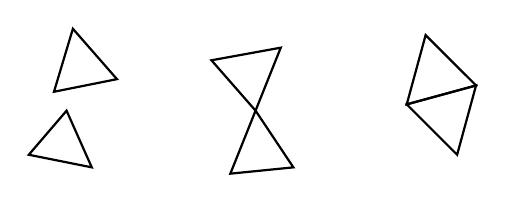
\begin{tikzpicture}[scale=0.8]
            \begin{scope}[shift={(0,0)}]
                \draw[thick] (0.8, 1.4) -- (1.8, 1.6) -- (1.1, 2.4) -- cycle;
                \draw[thick] (0.4, 0.4) -- (1.4, 0.2) -- (1.0, 1.1) -- cycle;
            \end{scope}
    
            \begin{scope}[shift={(3.0,0)}] 
                \coordinate (Center) at (1.0, 1.1);
                \draw[thick] (Center) -- (0.3, 1.9) -- (1.4, 2.1) -- cycle;
                \draw[thick] (Center) -- (0.6, 0.1) -- (1.6, 0.2) -- cycle;
            \end{scope}
    
            \begin{scope}[shift={(6.0,0)}]
                \coordinate (Left) at (0.4, 1.2);
                \coordinate (Right) at (1.5, 1.5);
                \draw[thick] (Left) -- (Right) -- (0.7, 2.3) -- cycle;
                \draw[thick] (Left) -- (Right) -- (1.2, 0.4) -- cycle;
            \end{scope}
        \end{tikzpicture}
        \caption{三种位置关系}
    \end{figure}
    
    这种情况下涉及 4 个点，5 条边。
    \begin{align*}
        \E[I_{ijk}I_{i^{\prime}j^{\prime}k^{\prime}}] &= p^{5} \\
        \text{Cov}(I_{ijk}, I_{i^{\prime}j^{\prime}k^{\prime}}) &= p^{5} - p^{3} \cdot p^{3} \approx p^{5}
    \end{align*}
    而这样的形状有 $\binom{n}{4}$ 个，所以
    \begin{align*}
        \Var(X) &= \sum \Var(I_{ijk}) + \sum \text{Cov}(I_{ijk}, I_{i^{\prime}j^{\prime}k^{\prime}}) \\
        &\approx \binom{n}{3} \cdot p^{3} + \binom{n}{4} \cdot p^{5} \\
        &\approx (np)^{3} + n^{4}p^{5}
    \end{align*}
    计算比值：
    \begin{align*}
        \frac{\Var(X)}{\E[X]^{2}} &\approx \frac{(np)^{3} + n^{4}p^{5}}{(np)^{6}} \\
        &= \frac{1}{(np)^3} + \frac{1}{n^2 p} \to 0
    \end{align*}
    $\therefore \Pr[X=0] \to 0$。
    即 $\Pr[\text{存在三角形}] \to 1$。
\end{proof}

作业题中存在更多的例子，比如 $G_{n,p}$ 中存在孤立点的概率（成为了期末考试题），图是二部图的概率，图中存在 $K_4$ 的概率（隔壁离散的期末题，那边介绍的更严谨，还有 sharp threshold 和 super sharp threshold 等）。

\end{document}